\documentclass[tikz,border=15pt]{standalone}
\usepackage{amsmath,amssymb}
\usetikzlibrary{calc,arrows.meta}

\begin{document}
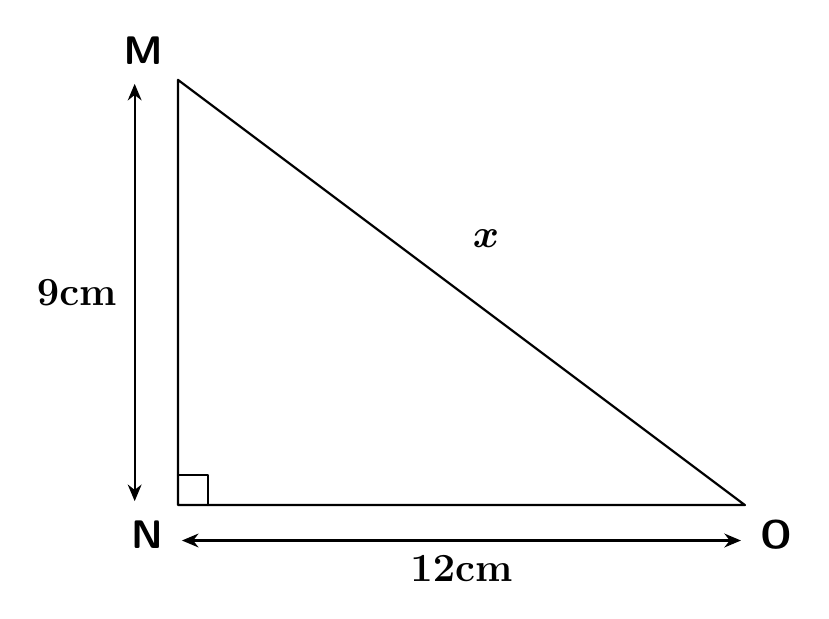
\begin{tikzpicture}[>=latex, line cap=round, line join=round]
  % Coordinates for exact 9:12:15 ratio rendered at 0.6 cm per unit
  % (adapted from diagram_24 template: 5-12-13 scale ruler applied to 9-12-x)
  \coordinate (N) at (0, 0);
  \coordinate (M) at (0, 5.4);
  \coordinate (O) at (7.2, 0);

  % Triangle boundary
  \draw[thick] (N) -- (M) -- (O) -- cycle;

  % Right-angle square at N
  \draw[thick] (0, 0.38) -- (0.38, 0.38) -- (0.38, 0);

  % Left vertical dimension line (9 cm)
  \draw[{Stealth[length=6pt, width=5pt]}-{Stealth[length=6pt, width=5pt]}, thick] (-0.55, 0.05) -- (-0.55, 5.35);
  \node[left=3pt] at (-0.55, 2.7) {\Large $\mathbf{9cm}$};

  % Bottom horizontal dimension line (12 cm)
  \draw[{Stealth[length=6pt, width=5pt]}-{Stealth[length=6pt, width=5pt]}, thick] (0.05, -0.45) -- (7.15, -0.45);
  \node[below=2pt] at (3.6, -0.45) {\Large $\mathbf{12cm}$};

  % Hypotenuse label: the unknown x
  \node[above right=2pt] at (3.55, 3.08) {\Large $\boldsymbol{x}$};

  % Vertices labels in bold sans-serif
  \node[above left=2pt, font=\Large\sffamily\bfseries] at (M) {M};
  \node[below left=2pt, font=\Large\sffamily\bfseries] at (N) {N};
  \node[below right=2pt, font=\Large\sffamily\bfseries] at (O) {O};
\end{tikzpicture}
\end{document}
